\newpage
\section{Задание 4.}

Сделать удобную замену переменных и найти площадь фигуры, выполнить
рисунок области.

$$    y = \frac{x^3}{a^2}, \quad y = \frac{x^3}{b^2}, \quad y = \frac{x^2}{c}, \quad y = \frac{x^2}{d}, \quad 0 < a < b, \quad 0 < c < d.$$

В идеале, нам нужно свести эту фигуру к прямоугольнику. Попробуем оставить параметры на одной части, переменные в другой.

$$ a^2 = \frac{x^3}{y}, \quad b^2 = \frac{x^3}{y}, \quad c = \frac{x^2}{y}, \quad d = \frac{x^2}{y}$$

Заметим, что для $a^2$ и $b^2$ уравнение повторяется, как и для $c$ и $d$.

$$ u = \dfrac{x^3}{y}\quad\quad v = \dfrac{x^2}{y} $$

Тогда эта область превращается в прямоугольник в $uv$ - плоскости, стороны которого ограничиваются сторонами $u=a^2$, $u=b^2$ и $v=c$ и $v=d$.

Можно посчитать площадь через следующий интеграл.

$$S = \int_{a^2}^{b^2} \int_{c}^{d} 1\cdot \left| \text{det}J\right| \,dv\,du$$

Где $\left|J\right|$ - это якобиан. Чтобы найти его, нужно выразить $x$ и $y$ через новые переменные. Сначала $x$.

$$
\begin{cases}
    u = \dfrac{x^3}{y}\,\vspace{1em}\\ 
    v = \dfrac{x^2}{y} 
\end{cases} \Rightarrow \quad
\begin{cases}
    y = \dfrac{x^3}{u}\,\vspace{1em}\\ 
    y = \dfrac{x^2}{v} 
\end{cases} \Rightarrow \quad
\dfrac{x^3}{u} = \dfrac{x^2}{v} \Rightarrow \quad
\dfrac{x^3}{x^2} = \dfrac{u}{v} \Rightarrow \quad
x = \dfrac{u}{v}
$$
Теперь $y$.
$$
\begin{cases}
    y = \dfrac{x^3}{u}\,\vspace{1em}\\ 
    x = \dfrac{u}{v}
\end{cases} \Rightarrow \quad 
y = \dfrac{u^3}{v^3} \cdot \dfrac{1}{u} = \dfrac{u^2}{v^3}
$$

Теперь посчитаем определитель якобиана.

$$\text{det}J = \text{det}\begin{pmatrix}
    \dfrac{\partial x}{\partial u} & \dfrac{\partial x}{\partial v} \vspace{1em}\\
    \dfrac{\partial y}{\partial u} & \dfrac{\partial y}{\partial v} 
\end{pmatrix}$$

$$\dfrac{\partial x}{\partial u} = \dfrac{\partial}{\partial u}\left(\dfrac{u}{v}\right) = \dfrac{1}{v} \quad\quad \dfrac{\partial x}{\partial v} = \dfrac{\partial}{\partial v}\left(\dfrac{u}{v}\right) = -\dfrac{u}{v^2}$$

$$\dfrac{\partial y}{\partial u} = \dfrac{\partial}{\partial u}\left( \dfrac{u^2}{v^3}\right) = \dfrac{2u}{v^3} \quad\quad \dfrac{\partial x}{\partial v} = \dfrac{\partial}{\partial v}\left(\dfrac{u^2}{v^3}\right) = -\dfrac{3u^2}{v^4}$$

Теперь подставим полученные значения в якобиан.

$$\text{det}\begin{pmatrix}
    \dfrac{\partial x}{\partial u} & \dfrac{\partial x}{\partial v} \vspace{1em}\\
    \dfrac{\partial y}{\partial u} & \dfrac{\partial y}{\partial v} 
\end{pmatrix} = \text{det}\begin{pmatrix}
    \dfrac{1}{v} & -\dfrac{u}{v^2} \vspace{1em}\\
    \dfrac{2u}{v^3} & -\dfrac{3u^2}{v^4}
\end{pmatrix} = \left( \frac{1}{v} \right) \left( -\frac{3u^2}{v^4} \right) - \left( -\frac{u}{v^2} \right) \left( \frac{2u}{v^3} \right) = \dfrac{u^2}{v^5}$$

Теперь вернемся к интегралу.

$$S = \int_{a^2}^{b^2} \int_{c}^{d} 1\cdot \left| \text{det}J\right| \,dv\,du = \int_{a^2}^{b^2} \int_{c}^{d} 1\cdot \left| - \dfrac{u^2}{v^5}\right| \,dv\,du = \int_{a^2}^{b^2} \int_{c}^{d} \dfrac{u^2}{v^5} \,dv\,du = $$

$$\int_{a^2}^{b^2} u^2 \,du\int_{c}^{d} \dfrac{1}{v^5} \,dv = \int_{a^2}^{b^2} u^2 \cdot \dfrac{1}{4v^4}\bigg|_{c}^d \,du = \int_{a^2}^{b^2} u^2 \dfrac{d^4 - c^4}{4c^4d^4} \,du = $$

$$= \dfrac{d^4 - c^4}{4c^4d^4} \int_{a^2}^{b^2} u^2 \,du = \dfrac{d^4 - c^4}{4c^4d^4} \cdot \dfrac{u^3}{3} \bigg|_{a^2}^{b^2} = \dfrac{d^4 - c^4}{4c^4d^4} \cdot \dfrac{b^6 - a^6}{3a^6b^6} =\boxed{\dfrac{(d^4 - c^4)(b^6 - a^6)}{12c^4d^4a^6b^6}}$$


\begin{figure}[h!t]
    \centering
    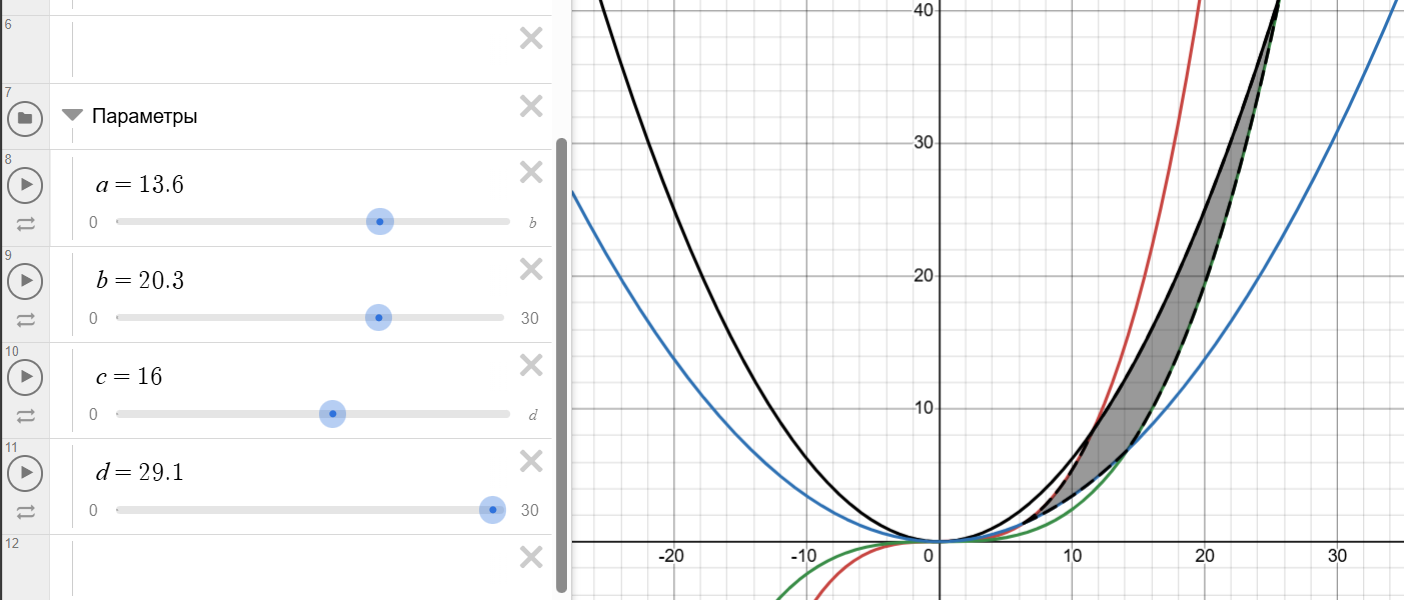
\includegraphics[width=1\linewidth]{Task4/graph.png}
    \caption{Задание 4. Изображение фигуры. \underline{\href{https://www.desmos.com/Calculator/5uewytafsp}{(Desmos)}}. }
\end{figure}